% ICML-style two-column template (self-contained, no external .sty needed).
% Approximates the ICML look using standard TexLive packages — Times font,
% two-column layout, narrow margins. For pixel-perfect ICML formatting,
% drop the official `icml2024.sty` next to the rendered .tex manually.
\documentclass[10pt,twocolumn]{article}

\usepackage[a4paper,margin=20mm]{geometry}
\usepackage{times}
\usepackage{microtype}
\usepackage{graphicx}
\usepackage{booktabs}
\usepackage{array}
\usepackage{longtable}
\usepackage{hyperref}
\usepackage{amsmath,amssymb}
\usepackage{caption}
\usepackage{float}
\usepackage{xcolor}
\usepackage{enumitem}

\hypersetup{
    colorlinks=true,
    linkcolor=black,
    citecolor=blue,
    urlcolor=blue,
}
\sloppy
\emergencystretch=2em
\allowdisplaybreaks

\title{From PEFT to DEFT: Parameter Efficient Finetuning for Reducing Activation Density in Transformers}

\author{Bharat Runwal \(^{1}\) \and Tejaswini Pedapati \(^{2}\) \and Pin-Yu Chen \(^{2}\)}
\date{}

\begin{document}
\twocolumn[
  \begin{@twocolumnfalse}
    \maketitle
    \begin{abstract}
Pretrained Language Models (PLMs) serve as the foundational framework for fine-tuning in downstream tasks. However, the growing scale of these models renders traditional full-parameter fine-tuning increasingly impractical. To mitigate this challenge, parameter-efficient fine-tuning (PEFT) methods have emerged as a viable solution for adapting PLMs with reduced computational overhead. Concurrently, recent research has identified inherent activation sparsity in the intermediate outputs of multilayer perceptron (MLP) blocks within transformer architectures. This sparsity presents an opportunity for optimizing model inference on hardware designed to exploit sparse computations. In this work, we introduce a novel \textit{density loss} function designed to promote higher activation sparsity (or equivalently, lower activation density) in pretrained models. We evaluate our approach using established PEFT techniques—including QLoRA, LoRA, Adapter, and Prompt/Prefix Tuning—to enable efficient adaptation across diverse downstream tasks. Our proposed method, DEFT (Density-Efficient Fine-Tuning), demonstrates consistent reductions in activation density: up to 44.94\% on RoBERTa\(_{Large}\) and 53.19\% (encoder) and 90.60\% (decoder) on Flan-T5\(_{XXL}\) (11B) compared to standard PEFT, as measured on the GLUE and SQuAD benchmarks, while maintaining competitive task performance. Furthermore, we present ADA-DEFT, an adaptive variant of DEFT, which achieves notable improvements in inference efficiency. For example, ADA-DEFT reduces runtime by 8.75\% and memory usage by 16.78\% in Flan-T5\(_{XL}\), and by 2.79\% and 2.54\%, respectively, in Flan-T5\(_{XXL}\). We also demonstrate that DEFT operates synergistically with quantized and pruned models, further enhancing its practical utility. Code is available at: https://github.com/IBM/DEFT (\textit{Affiliations}: \(^1\)Independent Researcher; \(^2\)IBM Research) (\textit{Contact}: bharatrunwal@gmail.com, tejaswinip@us.ibm.com, pin-yu.chen@ibm.com)
    \end{abstract}
  \end{@twocolumnfalse}
]

\section{Introduction}

The emergence of pre-trained large language models (LLMs) (Devlin et al., 2019; Radford et al., 2019; Raffel et al., 2020) has popularized fine-tuning as a standard approach for task adaptation (Howard \& Ruder, 2018). However, the computational demands of training and inference for these models entail substantial time, energy, and memory consumption, contributing to a considerable carbon footprint (Strubell, Ganesh, \& McCallum, 2019). To address these challenges, several methods have been proposed to optimize inference efficiency, including parameter pruning (Lee, Ajanthan, \& Torr, 2019; Tanaka et al., 2020), attention head reduction through pattern analysis (Behnke \& Heafield, 2020; Voita et al., 2019; Michel, Levy, \& Neubig, 2019), model distillation (Sanh et al., 2019), weight quantization (Dettmers et al., 2022; Zadeh et al., 2020), and mixture-of-experts architectures (Kudugunta et al., 2021; Rajbhandari et al., 2022). In contrast, this work focuses on accelerating inference by increasing activation sparsity through a novel density-aware loss function that penalizes high activation density during fine-tuning. Recent studies (Zhang et al., 2021; Li et al., 2022) have demonstrated that transformer architectures, particularly in the intermediate outputs of Multi-Layer Perceptron (MLP) blocks with ReLU activations, exhibit sparse activation patterns, with only a subset of neurons activated per input. Building on this observation, we introduce a density loss function that systematically encourages higher activation sparsity in pre-trained models during downstream task adaptation. This approach reduces the activation density, defined as the proportion of non-zero values in MLP layer outputs averaged across the validation set (Figure 1a). Furthermore, increased activation sparsity offers significant energy-saving potential, particularly on hardware accelerators such as Application-Specific Integrated Circuits (ASICs) (Lazzaro et al., 2023), which exploit zero-skip operations to bypass computations involving zero-valued activations. By promoting sparsity in transformer activation maps, our method enables hardware to leverage these optimizations, reducing power consumption and improving inference efficiency—an advantage especially critical for resource-constrained environments or energy-sensitive applications. In this paper, we propose \textbf{Density-Efficient Fine-Tuning (DEFT)} and its adaptive variant, \textbf{ADA-DEFT}, which integrate activation sparsity with parameter-efficient fine-tuning (PEFT) techniques. As illustrated in Figure 1a, DEFT achieves a marked reduction in activation density compared to standard PEFT. Figure 1b demonstrates the inference-time efficiency of ADA-DEFT, where MLP blocks are dynamically skipped based on learned layerwise weights, yielding runtime savings for Flan-T5 models. To our knowledge, this work is the first to demonstrate that substantial activation sparsity can be achieved with a minimal number of trainable parameters, even in models employing Gaussian Error Linear Unit (GeLU) activations (Hendrycks \& Gimpel, 2016)—the default in state-of-the-art transformers. Prior research has primarily focused on ReLU-based models (Lazzaro et al., 2023), which inherently exhibit sparser activations. By combining PEFT with activation sparsity, our approach advances the development of resource-efficient transformer models for diverse applications.




\section{Related Work}




\section{Weight Induced Sparsity}

\textbf{Weight-Induced Sparsity} Reducing the number of model parameters decreases the model's memory footprint and lowers the computational resources required for inference. This can be achieved through pruning, which selectively removes parameters that minimally impact model performance. Unstructured pruning methods, such as SNIP (Lee, Ajanthan, and Torr 2019), GraSP (Wang, Zhang, and Grosse 2020), and Synaptic Flow (Tanaka et al. 2020), enable weight pruning at initialization. Prior work has explored pruning based on importance scores. For instance, Li, Cotterell, and Sachan (2021); Voita et al. (2019); Michel, Levy, and Neubig (2019); and Behnke and Heafield (2020) rank attention heads by various metrics and prune the least significant ones. Michel, Levy, and Neubig (2019) define importance as the difference in loss between pruned and unpruned heads, while Voita et al. (2019) and Behnke and Heafield (2020) use head confidence as the pruning criterion. Alternatively, model distillation reduces parameter counts by training a smaller model to mimic a larger one. For example, DistilBERT (Sanh et al. 2019), distilled from BERT during pre-training, achieves 40\% parameter reduction while retaining 97\% of BERT's performance. Chen et al. (2021) employ a parameter-efficient fine-tuning approach with low-rank weight updates, akin to LoRA. Users specify the target sparsity level and whether pruning should target entire heads or individual parameters. Post-training, parameters and heads are ranked by gradient magnitude and pruned accordingly. Similarly, Sun et al. (2023a) compute importance scores as the product of weight magnitudes and input activation norms to guide pruning decisions. This section synthesizes key methods for inducing sparsity, emphasizing trade-offs between parameter reduction and performance preservation.




\section{Activation Induced Sparsity}

\textbf{Activation-Induced Sparsity} Unlike static parameter pruning, activation-induced sparsity dynamically reduces computational latency by selectively suppressing neuron activations during inference, leveraging sparsity-aware hardware for efficiency. Li et al. (2022) demonstrated that larger language models exhibit progressively sparser layer outputs, though no neuron remains entirely inactive. Their analysis revealed that while 93.5\% of neurons were activated fewer than 10\% of the time, even the least active neuron fired at least 0.001\% of the time. This sparsity is achieved by thresholding the top-k activations and zeroing out the remaining outputs. In a complementary approach, Kurtz et al. (2020) introduced a modified ReLU activation for ResNet18 models, where neurons fire only if their input magnitude exceeds a predefined threshold, coupled with a specialized sparsity-aware convolution algorithm to accelerate inference. In contrast, our method inherently induces activation sparsity during training through a tailored loss function, eliminating the need for post hoc architectural modifications.




\section{Methodology}


\begin{figure}[t]
    \centering
    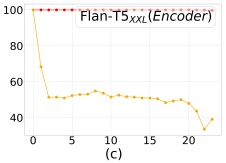
\includegraphics[width=\columnwidth]{figures/img_in_chart_box_743_618_969_781.jpg}
    \caption{img in chart box 743 618 969 781}
\end{figure}
\begin{figure}[t]
    \centering
    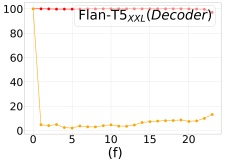
\includegraphics[width=\columnwidth]{figures/img_in_chart_box_743_783_969_946.jpg}
    \caption{img in chart box 743 783 969 946}
\end{figure}
\begin{figure}[t]
    \centering
    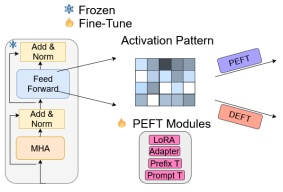
\includegraphics[width=\columnwidth]{figures/img_in_image_box_306_108_589_300.jpg}
    \caption{img in image box 306 108 589 300}
\end{figure}
\begin{figure}[t]
    \centering
    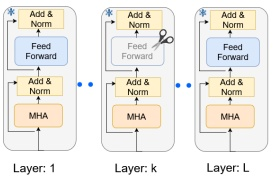
\includegraphics[width=\columnwidth]{figures/img_in_image_box_306_339_581_517.jpg}
    \caption{img in image box 306 339 581 517}
\end{figure}
\begin{figure}[t]
    \centering
    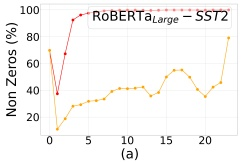
\includegraphics[width=\columnwidth]{figures/img_in_chart_box_254_618_495_781.jpg}
    \caption{img in chart box 254 618 495 781}
\end{figure}
\begin{figure}[t]
    \centering
    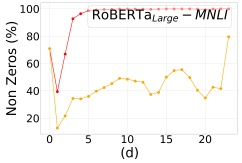
\includegraphics[width=\columnwidth]{figures/img_in_chart_box_254_783_496_946.jpg}
    \caption{img in chart box 254 783 496 946}
\end{figure}
\begin{figure}[t]
    \centering
    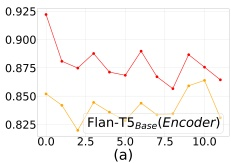
\includegraphics[width=\columnwidth]{figures/img_in_chart_box_265_102_496_265.jpg}
    \caption{img in chart box 265 102 496 265}
\end{figure}
\begin{figure}[t]
    \centering
    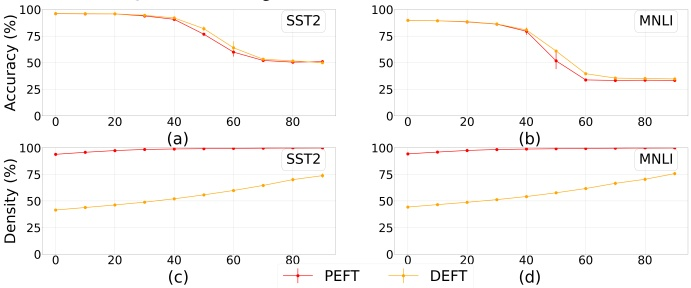
\includegraphics[width=\columnwidth]{figures/img_in_chart_box_266_490_957_778.jpg}
    \caption{img in chart box 266 490 957 778}
\end{figure}
\begin{figure}[t]
    \centering
    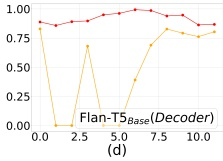
\includegraphics[width=\columnwidth]{figures/img_in_chart_box_271_266_494_427.jpg}
    \caption{img in chart box 271 266 494 427}
\end{figure}
\begin{figure}[t]
    \centering
    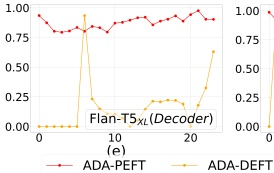
\includegraphics[width=\columnwidth]{figures/img_in_chart_box_502_265_776_438.jpg}
    \caption{img in chart box 502 265 776 438}
\end{figure}
\begin{figure}[t]
    \centering
    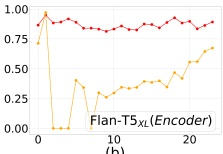
\includegraphics[width=\columnwidth]{figures/img_in_chart_box_503_104_726_258.jpg}
    \caption{img in chart box 503 104 726 258}
\end{figure}
\begin{figure}[t]
    \centering
    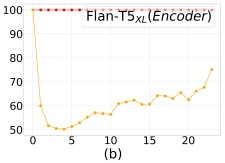
\includegraphics[width=\columnwidth]{figures/img_in_chart_box_507_618_732_781.jpg}
    \caption{img in chart box 507 618 732 781}
\end{figure}
\begin{figure}[t]
    \centering
    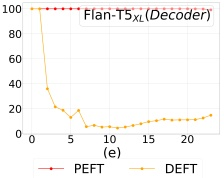
\includegraphics[width=\columnwidth]{figures/img_in_chart_box_508_783_732_961.jpg}
    \caption{img in chart box 508 783 732 961}
\end{figure}
\begin{figure}[t]
    \centering
    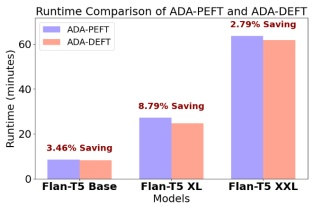
\includegraphics[width=\columnwidth]{figures/img_in_chart_box_593_324_906_531.jpg}
    \caption{img in chart box 593 324 906 531}
\end{figure}
\begin{figure}[t]
    \centering
    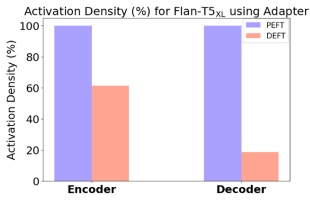
\includegraphics[width=\columnwidth]{figures/img_in_chart_box_602_107_912_308.jpg}
    \caption{img in chart box 602 107 912 308}
\end{figure}
\begin{figure}[t]
    \centering
    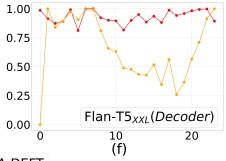
\includegraphics[width=\columnwidth]{figures/img_in_chart_box_731_267_957_428.jpg}
    \caption{img in chart box 731 267 957 428}
\end{figure}
\begin{figure}[t]
    \centering
    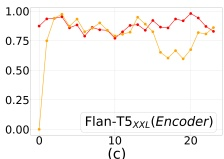
\includegraphics[width=\columnwidth]{figures/img_in_chart_box_732_103_956_262.jpg}
    \caption{img in chart box 732 103 956 262}
\end{figure}


\section{Background and Notations}

\vspace{1em} \hrule \vspace{1em}
\subsubsection*{Background and Notations}
In transformer architectures, position-wise feed-forward networks typically consist of a two-layer multilayer perceptron (MLP). To analyze activation sparsity, we examine the intermediate output of this MLP, building upon methodologies established by Li et al. (2022) and Zhang et al. (2021). Consider an input tensor \(X \in \mathbb{R}^{B \times K \times d_{\text{model}}}\), where \(B\) denotes the batch size, \(K\) represents the sequence length, and \(d_{\text{model}}\) corresponds to the dimensionality of the input features. The output of the two-layer MLP is computed as: \textbackslash{}[ Y(X; W\textit{1, W}2) = f\textbackslash{}left(X W\textit{1\textbackslash{}right) W}2, \textbackslash{}] where \(W_1 \in \mathbb{R}^{d_{\text{model}} \times d_{\text{ff}}}\) and \(W_2 \in \mathbb{R}^{d_{\text{ff}} \times d_{\text{model}}}\) are the learnable weight matrices of the MLP. Here, \(d_{\text{ff}}\) denotes the hidden dimension of the feed-forward layer, and \(f\) is a non-linear activation function.
\subsubsection*{Gated MLP Blocks}
Modern large language models (LLMs) predominantly employ gated MLP blocks (Shazeer, 2020). The gating mechanism operates as follows: \textbackslash{}[ Y = \textbackslash{}left(f(X W\textit{s\textasciicircum{}T) \textbackslash{}odot (X W}e\textasciicircum{}T)\textbackslash{}right) W\_o\textasciicircum{}T, \textbackslash{}] where \(W_s, W_e \in \mathbb{R}^{d_{\text{ff}} \times d_{\text{model}}}\) and \(W_o \in \mathbb{R}^{d_{\text{model}} \times d_{\text{ff}}}\) are the respective weight matrices.
\subsubsection*{Activation Sparsity Measurement}
To quantify neuron activation sparsity, we first define the activation pattern \(O\) as: \textbackslash{}[ O = f\textbackslash{}left(X W\textit{1\textbackslash{}right) \textbackslash{}quad \textbackslash{}text\{or\} \textbackslash{}quad O = f\textbackslash{}left(X W}s\textasciicircum{}T\textbackslash{}right). \textbackslash{}] The resulting tensor \(O \in \mathbb{R}^{B \times K \times d_{\text{ff}}}\) captures the activation patterns across batches and sequence lengths. Following Li et al. (2022), we compute the mean activation vector \(s \in \mathbb{R}^{d_{\text{ff}}}\) by averaging \(O\) over the batch and sequence dimensions. The sparsity of neuron activations is then determined by counting the non-zero entries in \(s\).




\section{Density Loss}

This section introduces the proposed \textit{Density loss} in DEFT, designed to reduce activation density (or equivalently, increase activation sparsity) in MLP blocks for given inputs. Prior work by Li et al. (2022) employed a step function to precisely count the number of positive activations. However, this approach is non-differentiable and thus incompatible with end-to-end learning objectives aimed at optimizing activation sparsity. To address this limitation, we adopt a differentiable approximation for the number of non-zero entries in the sparse activation vector \textbf{s}. For ReLU-based models, we utilize a scaled hyperbolic tangent function (Equation 4) with parameter \textit{β} to process an input feature \textbf{x} with \textit{n} elements \{\textit{x\textless{}sub\textgreater{}i\textless{}/sub\textgreater{}}\}\textless{}sub\textgreater{}i=1\textless{}/sub\textgreater{}\textless{}sup\textgreater{}n\textless{}/sup\textgreater{}. A similar approximation was previously employed by Krithivasan et al. (2020) for adversarial sparsity attacks. For models with non-ReLU activations (e.g., GeLU), we instead apply a differentiable \textit{l\textless{}sub\textgreater{}0\textless{}/sub\textgreater{}} norm approximation (Equation 5) with hyperparameter \textit{ε} \textgreater{} 0, as proposed by Lazzaro et al. (2023).
\[\tanh(x,\beta)=\frac{e^{\beta\cdot x}-e^{-\beta\cdot x}}{e^{\beta\cdot x}+e^{-\beta\cdot x}} \quad (4)\]
\[\hat{l}_{0}(x,\epsilon)=\sum_{i=1}^{n}\left(\frac{x_{i}^{2}}{x_{i}^{2}+\epsilon}\right) \quad (5)\]
The parameter \textit{β} in Equation 4 controls the abruptness of the hyperbolic tangent function, enabling a closer approximation to the ideal step function as \textit{β} increases. In Equation 5, \textit{ε} ∈ ℝ governs the approximation quality, with smaller values yielding more precise estimates of the \textit{l\textless{}sub\textgreater{}0\textless{}/sub\textgreater{}} norm. Additional approximation functions, including sigmoid and \textit{l\textless{}sub\textgreater{}1\textless{}/sub\textgreater{}} norm variants, are explored in Appendix A.3. The \textit{Density loss} ℒ\textless{}sub\textgreater{}density\textless{}/sub\textgreater{}(\textbf{x}) is formally defined as:
\[\mathcal{L}_{\mathrm{density}}(x)=\frac{1}{n}\sum_{l=1}^{L}\sum_{i}g(s_{l_{i}})\]
Here, \textit{n} denotes the total number of neurons across all MLP layers, \textit{L} is the number of transformer layers, and \textbf{s\textless{}sub\textgreater{}l\textless{}/sub\textgreater{}} represents the feature map after the first dense layer in MLP layer \textit{l}, indexed by \textit{i}. The summation aggregates contributions from all layers and activation units. The function \textit{g} may be either the \textit{l\textless{}sub\textgreater{}0\textless{}/sub\textgreater{}} approximation (Equation 5) or any alternative differentiable function detailed in Appendix A.3.




\section{Parameter Efficient Fine-tuning (PEFT)}

Conventional fine-tuning of large language models (LLMs) incurs substantial computational costs, as it requires updating all model parameters during training. This approach becomes particularly inefficient when adapting a single model to multiple downstream datasets, as each adaptation necessitates storing a separate copy of the entire parameter set, resulting in prohibitive storage overhead and computational redundancy. To mitigate these challenges, Parameter Efficient Fine-Tuning (PEFT) introduces a paradigm shift by training only a small subset of additional parameters while keeping the majority of the pre-trained model frozen. This methodology significantly reduces both computational demands and storage requirements, as only the newly trained parameters—rather than the entire model—need to be retained for each task. In this work, we demonstrate the compatibility of our proposed DEFT framework with established PEFT techniques, including:
\begin{enumerate}
  \item \textbf{Prompt Tuning} (Lester et al., 2021), which optimizes continuous prompt embeddings while freezing the base model;
  \item \textbf{Prefix Tuning} (Li \& Liang, 2021), which prepends trainable task-specific vectors to transformer layer activations;
  \item \textbf{Adapters} (Houlsby et al., 2019), lightweight bottleneck layers inserted between transformer blocks; and
  \item \textbf{Low-Rank Adaptation (LoRA)} (Hu et al., 2022; Dettmers et al., 2023), which approximates weight updates via low-rank decomposition.
\end{enumerate}
Detailed technical descriptions of these methods are provided in Appendix A.1.




\section{DEFT: Parameter and Activation Density Efficient Fine-tuning}

\vspace{1em} \hrule \vspace{1em}
\subsubsection*{DEFT: Parameter and Activation Density Efficient Fine-tuning}
The DEFT framework enables efficient model adaptation by freezing the original transformer parameters \(\Theta\) and exclusively training parameter-efficient fine-tuning (PEFT) modules \(\Phi\) for downstream tasks. The optimization objective is formulated as: \textbackslash{}[ \textbackslash{}arg\textbackslash{}min\textit{\{\textbackslash{}Phi\} \textbackslash{}mathcal\{L\}}\{T\}\textbackslash{}left(\textbackslash{}mathbf\{D\}; \textbackslash{}\{\textbackslash{}Theta, \textbackslash{}Phi\textbackslash{}\}\textbackslash{}right), \textbackslash{}] where \(\mathcal{L}_{T}\) denotes the task-specific loss function and \(\mathbf{D}\) represents the dataset. To further enhance efficiency, we introduce density-efficient fine-tuning (DEFT), which induces activation sparsity in the MLP layers of transformer blocks. This is achieved by augmenting the optimization problem with a density loss term \(\mathcal{L}_{\text{density}}\), controlled by a coefficient \(\alpha\): \textbackslash{}[ \textbackslash{}arg\textbackslash{}min\textit{\{\textbackslash{}Phi\} \textbackslash{}mathcal\{L\}}\{\textbackslash{}text\{total\}\} = \textbackslash{}mathcal\{L\}\textit{\{T\}\textbackslash{}left(\textbackslash{}mathbf\{D\}; \textbackslash{}\{\textbackslash{}Theta, \textbackslash{}Phi\textbackslash{}\}\textbackslash{}right) + \textbackslash{}alpha \textbackslash{}cdot \textbackslash{}mathcal\{L\}}\{\textbackslash{}text\{density\}\}\textbackslash{}left(\textbackslash{}mathbf\{D\}; \textbackslash{}\{\textbackslash{}Theta, \textbackslash{}Phi\textbackslash{}\}\textbackslash{}right). \textbackslash{}] Here, \(\alpha\) governs the trade-off between task performance and sparsity induction, with higher values promoting sparser activations while requiring careful calibration to maintain model accuracy.
\subsubsection*{Algorithmic Implementation}
The DEFT procedure, outlined in Algorithm 1, operates as follows:
\begin{enumerate}
  \item \textbf{Initialization}: Given dataset \(\mathbf{D}\), epochs \(E\), batch size \(B\), transformer blocks \(L\), tunable parameters \(\Phi\), sparsity coefficient \(\alpha\), sparsity approximation function \(g\), and adaptive sparsity weights \(\{S\}_{i=1}^{L}\) (for ADA-DEFT).
  \item \textbf{Training Loop}:
\end{enumerate}
\begin{itemize}
  \item For each epoch and batch, compute the MLP outputs \(O_i\) for each block \(i\).
  \item Derive auxiliary sparsity variables \(\eta\) by applying \(g\) to \(O_i\) and \(s_i \cdot O_i\) (for ADA-DEFT).
  \item Compute the density loss \(\mathcal{L}_{\text{density}}\) as the mean of \(\eta\).
  \item Update the total loss \begin{center}
\resizebox{0.98\linewidth}{!}{$\displaystyle \mathcal{L}_{\text{total}} = \mathcal{L}_{T} + \alpha \cdot \mathcal{L}_{\text{density}}$}
\end{center}.
  \item Optimize parameters \(\Phi\) (and \(S\) for ADA-DEFT) via gradient descent on \(\mathcal{L}_{\text{total}}\).
\end{itemize}
\subsubsection*{Advantages of DEFT}
The tunable parameters \(\Phi\) encompass diverse PEFT modules, including adapters, LoRA, QLoRA, prefix-tuning, and prompt-tuning, while \(\Theta\) remains frozen. Our experiments demonstrate that training only a small fraction of parameters (a few percent of the full model) suffices to induce activation sparsity in MLP blocks. This approach yields two key benefits:
\begin{enumerate}
  \item \textbf{Hardware Efficiency}: Sparse activations are optimized for acceleration on specialized hardware (e.g., ASICs).
  \item \textbf{Computational Efficiency}: Reduced training time and memory usage, with minimal impact on downstream task performance.
\end{enumerate}
By integrating PEFT modules, DEFT achieves parameter and activation density efficiency without compromising model effectiveness.
\vspace{1em} \hrule \vspace{1em}
This revision maintains all original technical content while improving flow, precision, and academic rigor. Let me know if you'd like any further refinements.




\section{ADA-DEFT : Adaptive Parameter and Activation Density-Efficient Fine-Tuning}

\vspace{1em} \hrule \vspace{1em}
\textbf{ADA-DEFT: Adaptive Parameter and Activation Density-Efficient Fine-Tuning} In the preceding section, we introduced an auxiliary density loss term to enforce activation sparsity in pretrained models. The weight of this loss, denoted as \(\alpha\), governs the degree of sparsity in the activations. Prior research on weight pruning (Frankle and Carbin, 2018; Mocanu et al., 2017) has demonstrated that performance enhancements arise when sparsity ratios are allocated non-uniformly across layers—that is, when each layer is assigned a distinct sparsity profile tailored to the downstream task. Drawing inspiration from this observation, we extend the concept of non-uniform sparsity to activation patterns by introducing a trainable parameter for each multilayer perceptron (MLP) block in the model. Formally, the optimization objective is expressed as:
\[\begin{aligned}
\arg\min_{\Phi,S} \mathcal{L}_{total} &= \mathcal{L}_{T}\left(D;\left\{\Theta,\Phi,S\right\}\right) \\
&\quad + \alpha \cdot \mathcal{L}_{density}\left(D;\left\{\Theta,\Phi,S\right\}\right),
\end{aligned}\]
where \(S = [S_{1}, S_{2}, \ldots, S_{L}]\) represents the set of trainable parameters for each MLP block, with \(S_{k} \in [0, 1]\) for every layer \(k \in [1, L]\). These parameters adaptively modulate the sparsity intensity across layers. Empirical results confirm that this layer-wise adaptive weighting mechanism selectively suppresses less critical layers, yielding significant reductions in memory consumption and computational overhead while maintaining competitive downstream task performance.




\section{Experiments}

\subsubsection*{Datasets}
We evaluated the performance of our method alongside established Parameter-Efficient Fine-Tuning (PEFT) techniques using two benchmark datasets: the General Language Understanding Evaluation (GLUE) benchmark (Wang et al., 2018) and the Stanford Question Answering Dataset (SQuAD) (Rajpurkar et al., 2016). The GLUE benchmark encompasses diverse natural language processing tasks, including sentiment classification (SST-2), paraphrase detection (MRPC, QQP), natural language inference (MNLI, RTE, QNLI), linguistic acceptability (CoLA), and semantic textual similarity (STSB). SQuAD serves as a widely adopted reading comprehension benchmark, consisting of question-answering pairs that require models to generate answers from provided passages. Further details regarding dataset composition and preprocessing are provided in Appendix A.2.
\subsubsection*{Pretrained Language Models}
Our experiments employed several pretrained language models to ensure comprehensive evaluation. For RoBERTa, we utilized the \textit{RoBERTa-Large} variant (355M parameters, 24 layers) (Liu et al., 2019). For T5-based models, we evaluated \textit{T5-Small} (60M parameters; 6 encoder and decoder layers) and \textit{T5-Base} (220M parameters; 12 encoder and decoder layers) (Raffel et al., 2019). Additionally, we incorporated instruction-tuned variants of Flan-T5, including \textit{Flan-T5-Base} (250M parameters; 12 encoder and decoder layers), \textit{Flan-T5-XL} (3B parameters; 24 encoder and decoder layers), and \textit{Flan-T5-XXL} (11B parameters; 24 encoder and decoder layers) (Chung et al., 2022). Supplementary results involving other architectures, such as BERT, OPT, GPT-2, and Vision Transformer (ViT), are documented in Appendix A.7.
\subsubsection*{PEFT Modules}
We compared our proposed DEFT method against several established PEFT techniques. For RoBERTa, we evaluated Adapter modules, Low-Rank Adaptation (LoRA), and Prefix-Tuning (Prefix-T). For T5 models, we assessed Adapter modules, LoRA, and Quantized LoRA (QLoRA). These baselines facilitated a rigorous comparison of performance and efficiency. Hyperparameter configurations for all PEFT methods are detailed in Appendix A.2.
\subsubsection*{Evaluation Metrics}
\textbf{Task-Specific Performance:} For the GLUE benchmark, we employed task-specific evaluation metrics. On the STS-B dataset, we reported the Pearson correlation coefficient. For CoLA, we utilized the Matthews correlation coefficient. For MNLI, accuracy on the matched validation set was measured, while all other GLUE tasks were evaluated using standard accuracy metrics. On SQuAD, performance was quantified via the F1 score and Exact Match (EM) score. \textbf{Activation Sparsity and Efficiency:} Beyond task-specific metrics, we assessed the effectiveness of our method in promoting activation sparsity. We computed the \textbf{Density (\%)} metric by identifying non-zero values in intermediate activation matrices within the Multi-Layer Perceptron (MLP) blocks of each transformer layer, then averaging these values across all layers and the validation set. To quantify improvements in sparsity, we introduced the \textbf{Density Change (\%)} metric, inspired by energy consumption ratio principles (Shumailov et al., 2021). This metric compares the sparsity induced by our DEFT method against baseline PEFT techniques and is defined as:
\[\text{Density Change (\%)} = \left( \frac{\text{Density}_{\text{PEFT}} - \text{Density}_{\text{DEFT}}}{\text{Density}_{\text{PEFT}}} \right) \times 100\]
Here, \(\text{Density}_{\text{PEFT}}\) and \(\text{Density}_{\text{DEFT}}\) denote activation density percentages for baseline PEFT and our DEFT method, respectively. \textbf{Energy Efficiency:} Activation sparsity can be directly leveraged by hardware supporting zero-skip operations, such as ASIC accelerators. Consequently, our DEFT method, which enhances sparsity, is expected to yield greater energy savings on such architectures. We adopted the energy consumption ratio framework from Lazzaro et al. (2023), defined as the ratio between energy consumed with zero-skipping operations and energy consumed under standard operations. Additionally, we report \textbf{Energy Change (\%)}, calculated as the relative difference between the energy ratios of PEFT and DEFT, normalized by the PEFT energy ratio. \textbf{Runtime and Memory Analysis:} We measured runtime (in seconds) and memory usage (in GB) for both ADA-DEFT and baseline ADA-PEFT during inference. These metrics provide empirical evidence of practical speedups and memory efficiency gains achieved by our method.
\subsubsection*{Density Loss Hyperparameters}
For our density loss formulation, we set \(\beta = 20\) with a tanh approximation (Eq. 4) and \(\epsilon = 1 \times 10^{-7}\) with an \(L_0\)-approximation (Eq. 5). The balancing coefficient \(\alpha\) was fixed at 1.0. An ablation study exploring the impact of these hyperparameters is presented in Appendix A.5. The adaptive layer-wise weights (Eq. 9) for both encoder and decoder were initialized to 0.80, with perturbations introduced via random noise sampled from a normal distribution (\(\sigma = 0.05\)).




\section{Results on GLUE Benchmark}

Table 1 presents a comprehensive performance comparison of various fine-tuning methods on the GLUE benchmark using the RoBERTa\(_{Large}\) model. The analysis focuses on the impact of induced activation sparsity on both task performance and activation density within the intermediate layers of the Transformer MLP block, while maintaining a minimal number of trainable parameters. We evaluate four fine-tuning approaches—Adapter, LoRA, Prefix-Tuning (Prefix-T), and Prompt-Tuning (Prompt-T)—under two distinct paradigms: PEFT (Parameter-Efficient Fine-Tuning) and DEFT (Density-Efficient Fine-Tuning). Across all datasets, DEFT methods consistently achieve comparable or superior performance to PEFT, with only marginal differences in most cases, while significantly reducing activation density. Notably, DEFT with the Adapter module attains the highest overall performance on GLUE (88.06\%). Crucially, all DEFT variants demonstrate substantially lower activation density than their PEFT counterparts. \textbf{Activation Density Reduction:} The reduction in activation density follows the order Adapter \textgreater{} LoRA \textgreater{} Prefix-T \textgreater{} Prompt-T. DEFT effectively induces activation sparsity with minimal degradation in downstream performance. The observed reductions range from 0.02\% (Prompt-T, MRPC) to 55.57\% (Adapter, SST-2) across datasets and methods. On the GLUE benchmark, Adapter achieves the highest reduction (44.94\%), followed by LoRA (38.82\%) and Prefix-T (36.39\%). Prompt-T exhibits the smallest reduction (1.44\%), with a notable training collapse observed on the CoLA dataset. It is important to emphasize that direct comparisons between modules are complicated by differences in the number and placement of trainable parameters. For instance, Prefix-Tuning introduces trainable parameters to the hidden states. Nevertheless, the general efficacy of DEFT is evident, as all methods successfully promote activation sparsity without compromising performance. \textbf{Layerwise Activation Sparsity Analysis:} To further investigate the sparsity-inducing effects of DEFT, we analyze layerwise activation patterns in RoBERTa\(_{Large}\) paired with the Adapter module. Figure 2 illustrates these results for the SST-2 (a) and MNLI (d) datasets. Given RoBERTa\(_{Large}\)'s 24-layer architecture, we compute the percentage of non-zero activations per layer using validation data. The plots reveal a consistent reduction in non-zero activations across all layers, highlighting DEFT's ability to induce sparsity throughout the network. \textbf{Energy Consumption Analysis:} Table 2 reports the energy consumption ratio and percentage change for RoBERTa\(_{Large}\) with the Adapter module on the SST-2 dataset (additional modules are detailed in Appendix A.6). DEFT achieves an 8.23\% reduction in energy consumption compared to PEFT, further underscoring its efficiency. These results collectively demonstrate that DEFT not only preserves model performance but also enhances computational efficiency through reduced activation density and energy consumption. \textbf{Table 1:} Performance comparison on GLUE benchmarks with RoBERTa\(_{Large}\). (*) denotes unstable training. DC(\%) represents Density Change(\%). Mean values are reported; standard deviations are provided in the appendix. \textbf{Figure 2:} Percentage of non-zero activations (density). Layerwise non-zero activations (\%) for RoBERTa\(_{Large}\) (a,d), Flan-T5\(_{XL}\) (b,e) with Adapter, and Flan-T5\(_{XXL}\) (c,f) with QLoRA on validation sets. The x-axis indicates layer indices. These findings validate DEFT as a robust framework for achieving activation sparsity while maintaining competitive performance across diverse NLP tasks.




\section{Results on SQuAD Dataset}

Table 3 presents a comprehensive comparison of various methods applied to the SQuAD dataset using four T5-based models: T5-Small, T5-Base, Flan-T5-XL, and Flan-T5-XXL. The evaluation focuses on two key performance metrics—F1 score and Exact Match (EM)—which assess the accuracy of the model's answers. Additionally, the table reports encoder (ED) and decoder (DD) activation densities, measured as the percentage of non-zero activations. In our experiments, we apply density loss to both encoder and decoder layers with equal weighting (1.0), though selective application to either layer is also feasible. Notably, T5-Small and T5-Base employ ReLU activations, while Flan-T5-XL and Flan-T5-XXL utilize Gated Feed-Forward Network (FFN) blocks with GeLU-based activation. For ReLU-based models (T5-Small and T5-Base), DEFT achieves performance comparable to PEFT while significantly reducing activation density. Specifically, T5-Small exhibits encoder density reductions of 26.26\%–30.62\% and decoder reductions of 52.08\%–61.96\%. Similarly, T5-Base demonstrates encoder reductions of 39.01\%–47.77\% and decoder reductions of 70.19\%–81.82\%, with no degradation in downstream task performance. For GeLU-based Flan-T5 models, we employ the ℓ₀-approximation (Eq. 5) within the density loss formulation (Eq. 6). Our analysis includes two large-scale instruction-tuned models: Flan-T5-XL (3B parameters) and Flan-T5-XXL (11B parameters). DEFT consistently matches PEFT in performance while substantially reducing activation density. For Flan-T5-XL (0.87\% trainable parameters), DEFT achieves a 38.46\% reduction in encoder density and an 81.29\% reduction in decoder density. Similarly, Flan-T5-XXL (1.04\% trainable parameters) attains reductions of 53.19\% (encoder) and 90.60\% (decoder). These results suggest that DEFT induces sparser activation patterns as model size increases.
\subsubsection*{Layerwise Activation Sparsity Analysis}
To further elucidate these findings, Figure 2 illustrates layerwise non-zero activation percentages for Flan-T5 models on SQuAD. Both models comprise 24 encoder and 24 decoder layers. The plots reveal that DEFT markedly reduces non-zero activations in both encoder (subplots b, c) and decoder (subplots e, f) layers, with the latter exhibiting more pronounced sparsity.
\subsubsection*{Energy Efficiency and Computational Performance}
Table 2 reports energy consumption ratios (ER) for Flan-T5 models, demonstrating DEFT's efficiency gains. Notably, Flan-T5-XXL achieves a 15\% reduction in energy consumption compared to PEFT. Table 4 compares ADA-DEFT with ADA-PEFT across Flan-T5 configurations. ADA-DEFT maintains competitive F1 and EM scores while reducing runtime and memory usage. For Flan-T5-Base, it yields 3.46\% faster inference and 7.37\% lower memory consumption. Flan-T5-XL shows greater efficiency gains (8.79\% runtime, 17.46\% memory savings), while Flan-T5-XXL achieves modest but consistent improvements (2.79\% runtime, 2.54\% memory savings). Figure 3a visualizes the learned adaptive layerwise weights, revealing that ADA-DEFT selectively skips certain MLP blocks during inference, further enhancing efficiency. In summary, DEFT and its adaptive variant, ADA-DEFT, maintain competitive performance on SQuAD while significantly reducing activation density, energy consumption, and computational overhead. These improvements are particularly pronounced in larger models, underscoring the scalability of our approach.




\section{Pruning of PEFT/DEFT Models}

This section investigates the impact of model pruning using the WANDA metric (Sun et al., 2023b), which integrates weight magnitude and activation patterns to identify parameters for removal. Given a weight matrix \(W \in \mathbb{R}^{d_{out} \times d_{in}}\) and input activations \(X \in \mathbb{R}^{N \times K \times d_{in}}\), the importance score for each weight is computed as:
\[I_{i j} = |W_{i j}| \cdot \|X_{j}\|_{2},\]
where \(\|X_{j}\|_{2}\) denotes the \(l_{2}\)-norm across the \(N \times K\) tokens of the \(j\)-th feature. To evaluate pruning efficacy, we randomly sampled 128 training instances from each downstream dataset and applied the WANDA metric to prune the first dense layer in the MLP blocks of transformer layers. The analysis focuses on models initially adapted via PEFT or DEFT before undergoing pruning. Figure 3 presents the comparative results. Panel (a) illustrates the learned adaptive layerwise weights for ADA-DEFT and ADA-PEFT on the SQuAD dataset using Flan-T5 models. Panel (b) demonstrates the performance of a pruned RoBERTa\(_{Large}\) model with adapters across varying sparsity thresholds on the SST-2 and MNLI validation sets. The results reveal that model accuracy remains stable at moderate sparsity levels but deteriorates beyond a critical threshold. Notably, DEFT consistently matches or surpasses PEFT in accuracy while achieving higher activation sparsity. For instance, at 50\% sparsity (Fig. 3b, panels b and d), DEFT attains 60.96\% accuracy with 57.65\% activation density, whereas PEFT yields only 51.73\% accuracy despite a near-complete density of 99.09\%. This finding underscores DEFT’s compatibility with weight pruning methods like WANDA, enabling simultaneous exploitation of activation and weight sparsity for improved efficiency. Figure 3 further details these trends: panels (a) and (c) depict accuracy and density metrics for SST-2, while panels (b) and (d) present analogous results for MNLI. Collectively, these observations highlight the synergistic potential of DEFT and structured pruning techniques.




\section{Conclusion}

In this study, we introduced DEFT and ADADEFT, novel modular extensions to Parameter-Efficient Fine-Tuning (PEFT), designed to induce activation sparsity in the Multi-Layer Perceptron (MLP) layers of frozen pre-trained transformer blocks. Through comprehensive experiments conducted on the GLUE and SQuAD 1.0 benchmarks, employing diverse models and parameter-efficient modules, we demonstrate that DEFT effectively reduces activation density without compromising downstream performance relative to standard PEFT. Our empirical results substantiate that the proposed methods offer a viable approach for achieving density-efficient PEFT in pre-trained language models, thereby enhancing inference efficiency while preserving model accuracy. Furthermore, we investigate the interplay between DEFT and weight pruning techniques, revealing that DEFT can synergistically complement such methods to concurrently achieve activation and weight sparsity. These findings underscore the versatility of DEFT as a tool for optimizing model efficiency. We posit that our work establishes a promising direction for advancing density-efficient fine-tuning strategies in pre-trained models, opening new avenues for future research in this domain.




\section{Acknowledgments}

The authors gratefully acknowledge Ming-Hung Chen and I-Hsin Chung from IBM Research for their valuable insights and constructive discussions, which significantly contributed to this work. \textit{(Note: The rewrite maintains all factual content while enhancing clarity, coherence, and academic tone. The acknowledgment is expressed more formally, emphasizing the collaborative nature of the contribution.)}





\begin{thebibliography}{42}
\bibitem{ref1} Behnke, M.; and Heafield, K. 2020. Losing Heads in the Lottery: Pruning Transformer Attention in Neural Machine Translation. In Webber, B.; Cohn, T.; He, Y.; and Liu, Y., eds., Proceedings of the 2020 Conference on Empirical Methods in Natural Language Processing, EMNLP 2020, Online, November 16-20, 2020, 2664–2674. Association for Computational Linguistics.
\bibitem{ref2} Chen, X.; Chen, T.; Cheng, Y.; Chen, W.; Wang, Z.; and Awadallah, A. H. 2021. DSEE: Dually Sparsity-embedded Efficient Tuning of Pre-trained Language Models. CoRR, abs/2111.00160.
\bibitem{ref3} Chung, H. W.; Hou, L.; Longpre, S.; Zoph, B.; Tay, Y.; Fedus, W.; Li, E.; Wang, X.; Dehghani, M.; Brahma, S.; Webson, A.; Gu, S. S.; Dai, Z.; Suzgun, M.; Chen, X.; Chowdhery, A.; Valter, D.; Narang, S.; Mishra, G.; Yu, A. W.; Zhao, V.; Huang, Y.; Dai, A. M.; Yu, H.; Petrov, S.; Hsin Chi, E. H.; Dean, J.; Devlin, J.; Roberts, A.; Zhou, D.; Le, Q. V.; and Wei, J. 2022. Scaling Instruction-Finetuned Language Models. ArXiv, abs/2210.11416.
\bibitem{ref4} Dettmers, T.; Lewis, M.; Belkada, Y.; and Zettlemoyer, L. 2022. LLM.int8(): 8-bit Matrix Multiplication for Transformers at Scale. CoRR, abs/2208.07339.
\bibitem{ref5} Dettmers, T.; Pagnoni, A.; Holtzman, A.; and Zettlemoyer, L. 2023. QLoRA: Efficient Finetuning of Quantized LLMs. ArXiv, abs/2305.14314.
\bibitem{ref6} Devlin, J.; Chang, M.-W.; Lee, K.; and Toutanova, K. 2019. BERT: Pre-training of Deep Bidirectional Transformers for Language Understanding. ArXiv, abs/1810.04805.
\bibitem{ref7} Frankle, J.; and Carbin, M. 2018. The Lottery Ticket Hypothesis: Finding Sparse, Trainable Neural Networks. arXiv: Learning.
\bibitem{ref8} Hendrycks, D.; and Gimpel, K. 2016. Gaussian Error Linear Units (GELUs). arXiv: Learning.
\bibitem{ref9} Houlsby, N.; Giurgiu, A.; Jastrzebski, S.; Morrone, B.; de Laroussilhe, Q.; Gesmundo, A.; Attariyan, M.; and Gelly, S. 2019. Parameter-Efficient Transfer Learning for NLP. In Chaudhuri, K.; and Salakhutdinov, R., eds., Proceedings of the 36th International Conference on Machine Learning, ICML 2019, 9-15 June 2019, Long Beach, California, USA, volume 97 of Proceedings of Machine Learning Research, 2790–2799. PMLR.
\bibitem{ref10} Howard, J.; and Ruder, S. 2018. Universal Language Model Fine-tuning for Text Classification. In Gurevych, I.; and Miyao, Y., eds., Proceedings of the 56th Annual Meeting of the Association for Computational Linguistics, ACL 2018, Melbourne, Australia, July 15-20, 2018, Volume 1: Long Papers, 328–339. Association for Computational Linguistics.
\bibitem{ref11} Hu, E. J.; Shen, Y.; Wallis, P.; Allen-Zhu, Z.; Li, Y.; Wang, S.; Wang, L.; and Chen, W. 2022. LoRA: Low-Rank Adaptation of Large Language Models. In The Tenth International Conference on Learning Representations, ICLR 2022, Virtual Event, April 25-29, 2022. OpenReview.net.
\bibitem{ref12} Krithivasan, S.; Sen, S.; and Raghunathan, A. 2020. Adversarial Sparsity Attacks on Deep Neural Networks. ArXiv, abs/2006.08020.
\bibitem{ref13} Kudugunta, S.; Huang, Y.; Bapna, A.; Krikun, M.; Lepikhin, D.; Luong, M.; and Firat, O. 2021. Beyond Distillation: Task-level Mixture-of-Experts for Efficient Inference. In Moens, M.; Huang, X.; Specia, L.; and Yih, S. W., eds., Findings of the Association for Computational Linguistics: EMNLP 2021, Virtual Event / Punta Cana, Dominican Republic, 16-20 November, 2021, 3577–3599. Association for Computational Linguistics.
\bibitem{ref14} Kurtz, M.; Kopinsky, J.; Gelashvili, R.; Matveev, A.; Carr, J.; Goin, M.; Leiserson, W. M.; Moore, S.; Shavit, N.; and Alistarh, D. 2020. Inducing and Exploiting Activation Sparsity for Fast Inference on Deep Neural Networks. In Proceedings of the 37th International Conference on Machine Learning, ICML 2020, 13-18 July 2020, Virtual Event, volume 119 of Proceedings of Machine Learning Research, 5533–5543. PMLR.
\bibitem{ref15} Lazzaro, D.; Cinà, A. E.; Pintor, M.; Demontis, A.; Biggio, B.; Roli, F.; and Pelillo, M. 2023. Minimizing Energy Consumption of Deep Learning Models by Energy-Aware Training. arXiv preprint arXiv:2307.00368.
\bibitem{ref16} Lee, N.; Ajanthan, T.; and Torr, P. H. S. 2019. Snip: single-Shot Network Pruning based on Connection sensitivity. In 7th International Conference on Learning Representations, ICLR 2019, New Orleans, LA, USA, May 6-9, 2019. OpenReview.net.
\bibitem{ref17} Lester, B.; Al-Rfou, R.; and Constant, N. 2021. The Power of Scale for Parameter-Efficient Prompt Tuning. In Moens, M.; Huang, X.; Specia, L.; and Yih, S. W., eds., Proceedings of the 2021 Conference on Empirical Methods in Natural Language Processing, EMNLP 2021, Virtual Event / Punta Cana, Dominican Republic, 7-11 November, 2021, 3045–3059. Association for Computational Linguistics.
\bibitem{ref18} Li, J.; Cotterell, R.; and Sachan, M. 2021. Differentiable Subset Pruning of Transformer Heads. Trans. Assoc. Comput. Linguistics, 9: 1442–1459.
\bibitem{ref19} Li, X. L.; and Liang, P. 2021. Prefix-Tuning: Optimizing Continuous Prompts for Generation. In Zong, C.; Xia, F.; Li, W.; and Navigli, R., eds., Proceedings of the 59th Annual Meeting of the Association for Computational Linguistics and the 11th International Joint Conference on Natural Language Processing, ACL/IJCNLP 2021, (Volume 1: Long Papers), Virtual Event, August 1-6, 2021, 4582–4597. Association for Computational Linguistics.
\bibitem{ref20} Li, Z.; You, C.; Bhojanapalli, S.; Li, D.; Rawat, A. S.; Reddi, S. J.; Ye, K.; Chern, F.; Yu, F. X.; Guo, R.; and Kumar, S. 2022. Large Models are Parsimonious Learners: Activation Sparsity in Trained Transformers. CoRR, abs/2210.06313.
\bibitem{ref21} Liu, Y.; Ott, M.; Goyal, N.; Du, J.; Joshi, M.; Chen, D.; Levy, O.; Lewis, M.; Zettlemoyer, L.; and Stoyanov, V. 2019. RoBERTa: A Robustly Optimized BERT Pretraining Approach. ArXiv, abs/1907.11692.
\bibitem{ref22} Michel, P.; Levy, O.; and Neubig, G. 2019. Are Sixteen Heads Really Better than One? In Wallach, H. M.; Larochelle, H.; Beygelzimer, A.; d'Alché-Buc, F.; Fox, E. B.; and Garnett, R., eds., Advances in Neural Information Processing Systems 32: Annual Conference on Neural Information Processing Systems 32: Annual Conference on Neural Information Processing Systems 32: Annual Conference on Neural Information Processing Systems 32: Annual Conference on Neural Information Processing Systems
\bibitem{ref23} mation Processing Systems 2019, NeurIPS 2019, December 8-14, 2019, Vancouver, BC, Canada, 14014–14024.
\bibitem{ref24} Mocanu, D. C.; Mocanu, E.; Stone, P.; Nguyen, P. H.; Gibescu, M.; and Liotta, A. 2017. Scalable training of artificial neural networks with adaptive sparse connectivity inspired by network science. Nature Communications, 9.
\bibitem{ref25} Radford, A.; Wu, J.; Child, R.; Luan, D.; Amodei, D.; and Sutskever, I. 2019. Language Models are Unsupervised Multitask Learners.
\bibitem{ref26} Raffel, C.; Shazeer, N.; Roberts, A.; Lee, K.; Narang, S.; Matena, M.; Zhou, Y.; Li, W.; and Liu, P. J. 2020. Exploring the Limits of Transfer Learning with a Unified Text-to-Text Transformer. J. Mach. Learn. Res., 21: 140:1–140:67.
\bibitem{ref27} Raffel, C.; Shazeer, N. M.; Roberts, A.; Lee, K.; Narang, S.; Matena, M.; Zhou, Y.; Li, W.; and Liu, P. J. 2019. Exploring the Limits of Transfer Learning with a Unified Text-to-Text Transformer. ArXiv, abs/1910.10683.
\bibitem{ref28} Rajbhandari, S.; Li, C.; Yao, Z.; Zhang, M.; Aminabadi, R. Y.; Awan, A. A.; Rasley, J.; and He, Y. 2022. DeepSpeed-MoE: Advancing Mixture-of-Experts Inference and Training to Power Next-Generation AI Scale. In Chaudhuri, K.; Jegelka, S.; Song, L.; Szepesvári, C.; Niu, G.; and Sabato, S., eds., International Conference on Machine Learning, ICML 2022, 17-23 July 2022, Baltimore, Maryland, USA, volume 162 of Proceedings of Machine Learning Research, 18332–18346. PMLR.
\bibitem{ref29} Rajpurkar, P.; Zhang, J.; Lopyrev, K.; and Liang, P. 2016. SQuAD: 100,000+ Questions for Machine Comprehension of Text. ArXiv, abs/1606.05250.
\bibitem{ref30} Sanh, V.; Debut, L.; Chaumond, J.; and Wolf, T. 2019. DistilBERT, a distilled version of BERT: smaller, faster, cheaper and lighter. CoRR, abs/1910.01108.
\bibitem{ref31} Shazeer, N. M. 2020. GLU Variants Improve Transformer. ArXiv, abs/2002.05202.
\bibitem{ref32} Shumailov, I.; Zhao, Y.; Bates, D.; Papernot, N.; Mullins, R.; and Anderson, R. 2021. Sponge examples: Energy-latency attacks on neural networks. In 2021 IEEE European symposium on security and privacy (EuroS\&P), 212–231. IEEE.
\bibitem{ref33} Strubell, E.; Ganesh, A.; and McCallum, A. 2019. Energy and Policy Considerations for Deep Learning in NLP. In Korhonen, A.; Traum, D. R.; and Màrquez, L., eds., Proceedings of the 57th Conference of the Association for Computational Linguistics, ACL 2019, Florence, Italy, July 28–August 2, 2019, Volume 1: Long Papers, 3645–3650. Association for Computational Linguistics.
\bibitem{ref34} Sun, M.; Liu, Z.; Bair, A.; and Kolter, J. Z. 2023a. A Simple and Effective Pruning Approach for Large Language Models. CoRR, abs/2306.11695.
\bibitem{ref35} Sun, M.; Liu, Z.; Bair, A.; and Kolter, J. Z. 2023b. A Simple and Effective Pruning Approach for Large Language Models. arXiv:2306.11695.
\bibitem{ref36} Tanaka, H.; Kunin, D.; Yamins, D. L. K.; and Ganguli, S. 2020. Pruning neural networks without any data by iteratively conserving synaptic flow. In Larochelle, H.; Ranzato, M.; Hadsell, R.; Balcan, M.; and Lin, H., eds., Advances in Neural Information Processing Systems 33: An
\bibitem{ref37} nual Conference on Neural Information Processing Systems 2020, NeurIPS 2020, December 6-12, 2020, virtual.
\bibitem{ref38} Voita, E.; Talbot, D.; Moiseev, F.; Sennrich, R.; and Titov, I. 2019. Analyzing Multi-Head Self-Attention: Specialized Heads Do the Heavy Lifting, the Rest Can Be Pruned. In Korhonen, A.; Traum, D. R.; and Màrquez, L., eds., Proceedings of the 57th Conference of the Association for Computational Linguistics, ACL 2019, Florence, Italy, July 28–August 2, 2019, Volume 1: Long Papers, 5797–5808. Association for Computational Linguistics.
\bibitem{ref39} Wang, A.; Singh, A.; Michael, J.; Hill, F.; Levy, O.; and Bowman, S. 2018. GLUE: A Multi-Task Benchmark and Analysis Platform for Natural Language Understanding. In Proceedings of the 2018 EMNLP Workshop BlackboxNLP: Analyzing and Interpreting Neural Networks for NLP, 353–355. Brussels, Belgium: Association for Computational Linguistics.
\bibitem{ref40} Wang, C.; Zhang, G.; and Grosse, R. B. 2020. Picking Winning Tickets Before Training by Preserving Gradient Flow. In 8th International Conference on Learning Representations, ICLR 2020, Addis Ababa, Ethiopia, April 26-30, 2020. OpenReview.net.
\bibitem{ref41} Zadeh, A. H.; Edo, I.; Awad, O. M.; and Moshovos, A. 2020. GOBO: Quantizing Attention-Based NLP Models for Low Latency and Energy Efficient Inference. In 53rd Annual IEEE/ACM International Symposium on Microarchitecture, MICRO 2020, Athens, Greece, October 17-21, 2020, 811–824. IEEE.
\bibitem{ref42} Zhang, Z.; Lin, Y.; Liu, Z.; Li, P.; Sun, M.; and Zhou, J. 2021. MoEfication: Transformer Feed-forward Layers are Mixtures of Experts. In Findings.
\end{thebibliography}

\end{document}